\documentclass[12pt]{article}

\usepackage{times}
\usepackage{textcomp}
\usepackage{listings}
\usepackage{fullpage}
\usepackage{color}
\usepackage{hyperref} 
\usepackage{pst-tree} 
\usepackage{verbatim} 
\usepackage{graphicx}
\usepackage{amsmath,amsfonts,amssymb,amsthm}
\graphicspath{ {./}}


\def\part#1{\item[\bf #1)]}
\renewcommand{\thesubsection}{Question \arabic{subsection}}

\author{Clement Tsang}

\begin{document}

\begin{center}
\Large\textbf{CS 241, Lecture 8 - Non-Deterministic Finite Automata}
\end{center}

\section{Non-Deterministic Finite Automata}
\begin{itemize}
    \item An \textbf{NFA} is a 5-tuple: $(\sigma, Q, q_0, A, \delta)$:
        \begin{itemize}
            \item $\Sigma$ is a finite non-empty set (alphabet)
            \item $Q$ is a finite non-empty set of states
            \item $q_0 \in Q$ is a start state
            \item $A \subseteq Q$ is a set of accepting states
            \item $\delta : (Q \times \Sigma) \rightarrow 2^Q$ is our total transition function, denoting ther \emph{power set} of $Q$
        \end{itemize}
    \item We can extend $\delta$ to $\delta^* : (2^Q \times \Sigma^*) \rightarrow 2^Q$:
        \begin{align*}
            \delta^* : (2^Q \times \Sigma^*) &\rightarrow 2^Q \\
            (S, \epsilon) &\rightarrow S \\
            (S, a) &\rightarrow \delta^* (\cup_{q\in S} \delta (q, a), w)
        \end{align*}
        where $a \in \Sigma$.  
    \item In other words, an NFA given by $M = (\Sigma, Q, q_0, A, \delta)$ \textbf{accepts a string} $w$ iff $\delta^* (\{q_0\}, w) \cup A \not= \varnothing$.
    \item This can be simulated like so with code:\\
        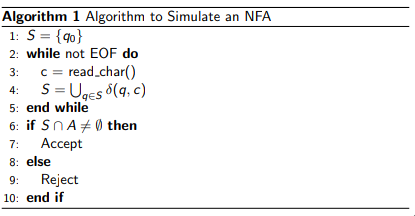
\includegraphics[scale=0.8]{nfa_simulate.png}
    \newpage
    \item For example, if $\Sigma = \{a, b\}, L = $ \{$w$ : $w$ ends with $bba$\}: \\
        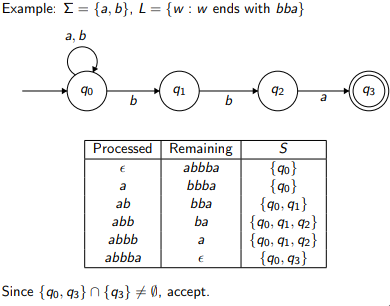
\includegraphics[scale=0.8]{abbba.png}
    \item To convert an NFA to a DFA, we start with state $S = \{q_0\}$.  We then go to the NFA and determine what happens on each $a \in \Sigma$ for each $q \in S$.  We repeat the previous step until we have every possibility.  Accepting states are any states that included an accepting state in the NFA.
    \item For example, the previous NFA as a DFA: \\
        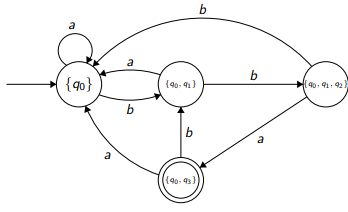
\includegraphics[scale=0.8]{nfa_as_dfa.png}
    \item Let us try another example.  Let $\Sigma = \{a, b, c\}$.  Write an NFA and DFA for the following examples:
        \begin{itemize}
            \item $L = \{abc\} \cup \{w : w \text{ ends with } cc\}$
            \item $L = \{abc\} \cup \{w : w \text{ contains } cc\}$
        \end{itemize}
    \item First example NFA: \\
        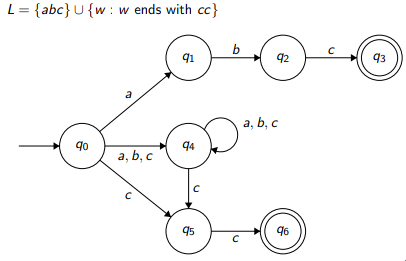
\includegraphics[scale=0.8]{nfa_ex1.png}
    \item First example DFA: \\
        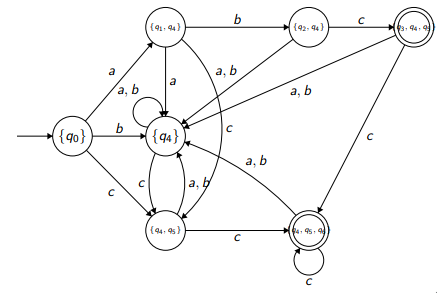
\includegraphics[scale=0.8]{dfa_ex1.png}
    \newpage
    \item Second example NFA: \\
        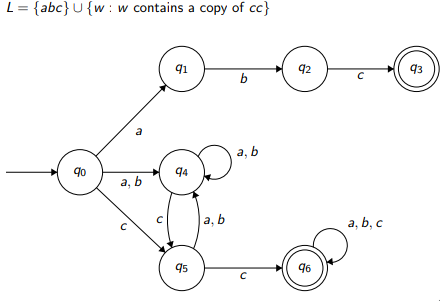
\includegraphics[scale=0.8]{nfa_ex2.png}
    \item Second example DFA: \\
        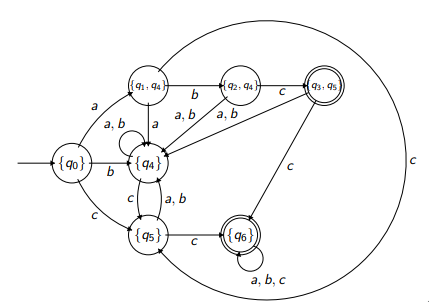
\includegraphics[scale=0.8]{dfa_ex2.png}
\end{itemize}

\newpage
\section{\texorpdfstring{$\epsilon$-NFA}{e-NFA}}
\begin{itemize}
    \item $\epsilon$ transitions are state changes without reading a character.
    \item We define a $\epsilon$-\textbf{NFA} is a 5-tuple $(\Sigma, Q, q_0, A, \delta)$:
        \begin{itemize}
            \item $\Sigma$ is a finite non-empty set (alphabet) that does \textbf{not} contain the symbol $\epsilon$
            \item $Q$ is a finite non-empty set of states
            \item $q_0 \in Q$ is a start state
            \item $A \subseteq Q$ is a set of accepting states
            \item $\delta : (Q \times \Sigma \cup \{\epsilon\}) \rightarrow 2^Q$ is our total transition function, where $2^Q$ denotes the power set of $Q$, the set of all subsets of $Q$
        \end{itemize}
    \item $\epsilon$-transitions make it trivial to take the union of two NFAs.  For example, for $L = \{abc\} \cup \{w : w \text{ ends with } cc\}$: \\
        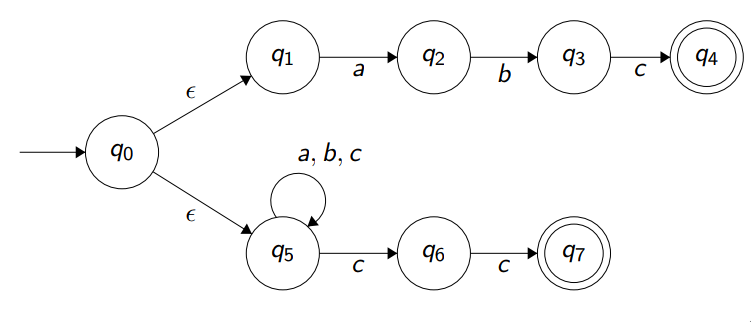
\includegraphics[scale=0.5]{ep-tran.png} \\
        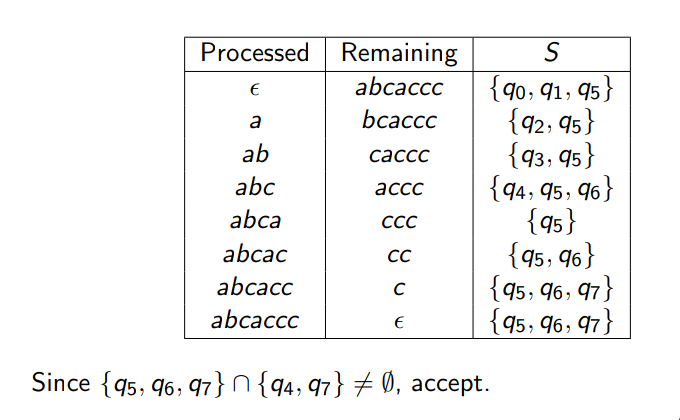
\includegraphics[scale=0.5]{ep-trace.png}
    \item If we were to let $E(S)$ to be the epsilon closure of a set of states $S$ (set of all states reachable from $S$ in 0 or more $\epsilon$-transitions.  This implies $S \subset E(S)$.
    \item We can simulate this like so: \\
        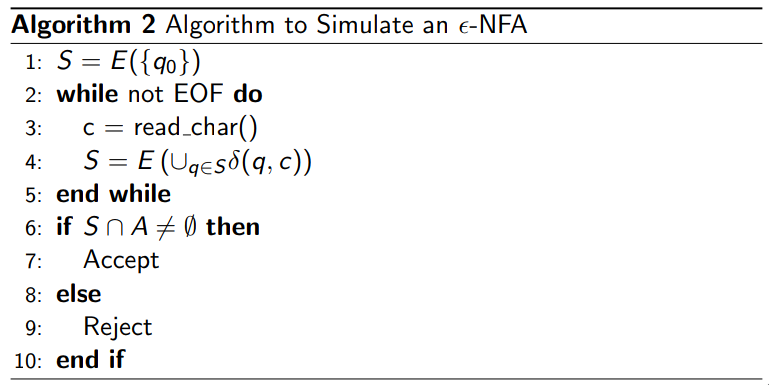
\includegraphics[scale=0.5]{e_nfa_sim.png}
    \item $epsilon$-NFAs that recognize regular languages:
        \begin{itemize}
            \item $\varnothing$
            \item $\{\epsilon \}$
            \item $\{a\}$
            \item $L_1 \cup L_2$ (that is, given $\epsilon$-NFAs that recognize $L_1$ and $L_2$ already, you can point $q_0$ to the two $L_1$ and $L_2$ machines)
            \item $L_1L_2$ (that is, given $\epsilon$-NFAs that recognize $L_1$ and $L_2$, you can point an accepting state in the $\epsilon-NFA$ of $L_1$ to the start state of $L_2$)
            \item $L^*$ (assume we have a $\epsilon$-NFA for $L$ already, then from each accepting state, add an $\epsilon$ transition back to the newly created start state
        \end{itemize}
    \item We can convert every $\epsilon$-NFA to a DFA, following the above technique for normal NFAs.
    \item By Kleene's Theorem, this implies every language recognized by an $\epsilon$-NFA is regular.
    \item We can do an example for the language $L$ of ID tokens in C: \\
        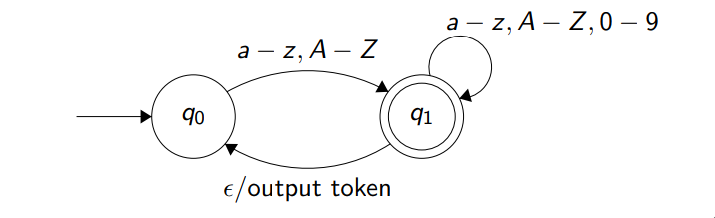
\includegraphics[scale=0.5]{c_id.png}
    \item But if we have the input of \emph{abcde}, we could get from 1 to 5 different tokens - what can we do?  We introduce maximal and simplified maximal munch
\end{itemize}

\section{Maximal Munch and Simplified Maximal Munch}
\begin{itemize}
    \item Maximal munch consumes characters until we no longer have a valid transition.  If we have characters left to consume, backtrack to the \emph{last} valid accepting state, and resume
    \item Simplified maximal munch consumes characters until we no longer have a valid transition.  If we are in an accepting state, produce the token and proceed.  Otherwise, go to an error state.
\end{itemize}

\end{document}

